\documentclass[10pt, twocolumn, letterpaper]{article}

%%%%%%%%% PAPER TYPE  - PLEASE UPDATE FOR FINAL VERSION
\usepackage{cvpr}
\usepackage{cite}
\usepackage{float}
              % To produce the CAMERA-READY version
% \usepackage[review]{cvpr}      % To produce the REVIEW version
% \usepackage[pagenumbers]{cvpr} % To force page numbers, e.g. for an arXiv version

% Import additional packages in the preamble file, before hyperref
\usepackage[dvipsnames]{xcolor}
\newcommand{\red}[1]{{\color{red}#1}}
\newcommand{\todo}[1]{{\color{red}#1}}
\newcommand{\TODO}[1]{\textbf{\color{red}[TODO:#1]}}


% It is strongly recommended to use hyperref, especially for the review version.
% hyperref with option pagebackref eases the reviewers' job.
% Please disable hyperref *only* if you encounter grave issues, 
% e.g. with the file validation for the camera-ready version.
%
% If you comment hyperref and then uncomment it, you should delete *.aux before re-running LaTeX.
% (Or just hit 'q' on the first LaTeX run, let it finish, and you should be clear).
\definecolor{cvprblue}{rgb}{0.21, 0.49, 0.74}
\usepackage[pagebackref,breaklinks,colorlinks,citecolor=cvprblue]{hyperref}
% \bibliographystyle{ieee}
% \bibliography{references}


%%%%%%%%% PAPER ID  - PLEASE UPDATE
\def\paperID{*****} % *** Enter the Paper ID here
\def\confName{CVPR}
\def\confYear{2024}

% It is strongly recommended to use hyperref, especially for the review version.
% hyperref with option pagebackref eases the reviewers' job.
% Please disable hyperref *only* if you encounter grave issues, 
% e.g. with the file validation for the camera-ready version.
%
% If you comment hyperref and then uncomment it, you should delete *.aux before re-running LaTeX.
% (Or just hit 'q' on the first LaTeX run, let it finish, and you should be clear).
\definecolor{cvprblue}{rgb}{0.21, 0.49, 0.74}
\usepackage[pagebackref,breaklinks,colorlinks,citecolor=cvprblue]{hyperref}
\usepackage{graphicx}
\usepackage{listings}
\usepackage{amsmath}

%%%%%%%%% PAPER ID  - PLEASE UPDATE
\def\paperID{*****} % *** Enter the Paper ID here
\def\confName{CVPR}
\def\confYear{2024}

%%%%%%%%% TITLE - PLEASE UPDATE
\title{
ML and DL Approaches to Galaxy Image Classification \\
\large{\normalfont EP4130: Data Science Analysis} \\
\normalfont Code: {\href{https://github.com/NamanChhibbar/EP4130-Project}{\textcolor {blue}{\normalfont https://github.com/NamanChhibbar/EP4130-Project}}}
terima k}

%%%%%%%% AUTHORS - PLEASE UPDATE
\author{
    Himanshu Jindal \\
    {\tt\small ma21btech11007@iith.ac.in}
    \and
    Naman Chhibbar \\
    {\tt\small ma21btech11011@iith.ac.in}
}

\begin{document}
\maketitle
\begin{abstract}
    We developed a dataset for classifying galaxy images into four categories: spiral, elliptical, irregular, and invalid. Using machine learning (ML) and deep learning (DL) techniques, including Support Vector Machines (SVM), Random Forest, Multi-Layer Perceptron (MLP), and Convolutional Neural Network (CNN), we automated galaxy classification. Our goal is to understand galaxy properties, such as star formation, using advanced ML and DL methods applied directly to the images.
\end{abstract}
   
\section{Introduction}
\label{sec:intro}

The Sloan Digital Sky Survey (SDSS) telescopes have collected a vast dataset of over 40TB of galaxy images. Classifying these images is crucial for understanding the physical processes within galaxies, including star formation and broader cosmological properties. Traditionally, this classification required manual analysis by expert astronomers. However, due to the lack of readily accessible datasets for galaxy classification, we compiled a dataset specifically tailored for this purpose.

Our project focuses on classifying galaxy images into four categories: spiral, elliptical, irregular, and invalid. We constructed a comprehensive dataset and evaluated its performance using various machine learning (ML) and deep learning (DL) algorithms. Initially, we applied Principal Component Analysis (PCA) to the dataset to reduce dimensionality and extract essential features. Subsequently, we employed a range of ML techniques, including Support Vector Machines (SVM) and Random Forest, and DL techniques, such as Multi-Layer Perceptron (MLP) and Convolutional Neural Network (CNN), directly on the images without PCA preprocessing.

Through this project, we aim to automate the galaxy classification process, facilitating a deeper understanding of these celestial objects using state-of-the-art ML and DL methods.
%-------------------------------------------------------------------------
% \subsection{Problem Statement}
% \subsection{Dual submission}

% Please refer to the author guidelines on the \confName\ \confYear\ web page for a
% discussion of the policy on dual submissions.

% \subsection{Paper length}
% Papers, excluding the references section, must be no longer than eight pages in length.
% The references section will not be included in the page count, and there is no limit on the length of the references section.
% For example, a paper of eight pages with two pages of references would have a total length of 10 pages.
% {\bf There will be no extra page charges for \confName\ \confYear.}

% Overlength papers will simply not be reviewed.
% This includes papers where the margins and formatting are deemed to have been significantly altered from those laid down by this style guide.
% Note that this \LaTeX\ guide already sets figure captions and references in a smaller font.
% The reason such papers will not be reviewed is that there is no provision for supervised revisions of manuscripts.
% The reviewing process cannot determine the suitability of the paper for presentation in eight pages if it is reviewed in eleven.

% %-------------------------------------------------------------------------
% \subsection{The ruler}
% The \LaTeX\ style defines a printed ruler which should be present in the version submitted for review.
% The ruler is provided in order that reviewers may comment on particular lines in the paper without circumlocution.
% If you are preparing a document using a non-\LaTeX\ document preparation system, please arrange for an equivalent ruler to appear on the final output pages.
% The presence or absence of the ruler should not change the appearance of any other content on the page.
% The camera-ready copy should not contain a ruler.
% (\LaTeX\ users may use options of \texttt{cvpr.sty} to switch between different versions.)

% Reviewers:
% note that the ruler measurements do not align well with lines in the paper --- this turns out to be very difficult to do well when the paper contains many figures and equations, and, when done, looks ugly.
% Just use fractional references (\eg, this line is $087.5$), although in most cases one would expect that the approximate location will be adequate.


% \subsection{Paper ID}
% Make sure that the Paper ID from the submission system is visible in the version submitted for review (replacing the ``*****'' you see in this document).
% If you are using the \LaTeX\ template, \textbf{make sure to update paper ID in the appropriate place in the tex file}.


% \subsection{Mathematics}

% Please number all of your sections and displayed equations as in these examples:
% \begin{equation}
%   E = m\cdot c^2
%   \label{eq:important}
% \end{equation}
% and
% \begin{equation}
%   v = a\cdot t.
%   \label{eq:also-important}
% \end{equation}
% It is important for readers to be able to refer to any particular equation.
% Just because you did not refer to it in the text does not mean some future reader might not need to refer to it.
% It is cumbersome to have to use circumlocutions like ``the equation second from the top of page 3 column 1''.
% (Note that the ruler will not be present in the final copy, so is not an alternative to equation numbers).
% All authors will benefit from reading Mermin's description of how to write mathematics:
% \url{http://www.pamitc.org/documents/mermin.pdf}.

% \subsection{Blind review}

% Many authors misunderstand the concept of anonymizing for blind review.
% Blind review does not mean that one must remove citations to one's own work---in fact it is often impossible to review a paper unless the previous citations are known and available.

% Blind review means that you do not use the words ``my'' or ``our'' when citing previous work.
% That is all.
% (But see below for tech reports.)

% Saying ``this builds on the work of Lucy Smith [1]'' does not say that you are Lucy Smith;
% it says that you are building on her work.
% If you are Smith and Jones, do not say ``as we show in [7]'', say ``as Smith and Jones show in [7]'' and at the end of the paper, include reference 7 as you would any other cited work.

% An example of a bad paper just asking to be rejected:
% \begin{quote}
% \begin{center}
%     An analysis of the frobnicatable foo filter.
% \end{center}

%    In this paper we present a performance analysis of our previous paper [1], and show it to be inferior to all previously known methods.
%    Why the previous paper was accepted without this analysis is beyond me.

%    [1] Removed for blind review
% \end{quote}


% An example of an acceptable paper:
% \begin{quote}
% \begin{center}
%      An analysis of the frobnicatable foo filter.
% \end{center}

%    In this paper we present a performance analysis of the  paper of Smith \etal [1], and show it to be inferior to all previously known methods.
%    Why the previous paper was accepted without this analysis is beyond me.

%    [1] Smith, L and Jones, C. ``The frobnicatable foo filter, a fundamental contribution to human knowledge''. Nature 381(12), 1-213.
% \end{quote}

% If you are making a submission to another conference at the same time, which covers similar or overlapping material, you may need to refer to that submission in order to explain the differences, just as you would if you had previously published related work.
% In such cases, include the anonymized parallel submission~\cite{Authors14} as supplemental material and cite it as
% \begin{quote}
% [1] Authors. ``The frobnicatable foo filter'', F\&G 2014 Submission ID 324, Supplied as supplemental material {\tt fg324.pdf}.
% \end{quote}

% Finally, you may feel you need to tell the reader that more details can be found elsewhere, and refer them to a technical report.
% For conference submissions, the paper must stand on its own, and not {\em require} the reviewer to go to a tech report for further details.
% Thus, you may say in the body of the paper ``further details may be found in~\cite{Authors14b}''.
% Then submit the tech report as supplemental material.
% Again, you may not assume the reviewers will read this material.

% Sometimes your paper is about a problem which you tested using a tool that is widely known to be restricted to a single institution.
% For example, let's say it's 1969, you have solved a key problem on the Apollo lander, and you believe that the 1970 audience would like to hear about your
% solution.
% The work is a development of your celebrated 1968 paper entitled ``Zero-g frobnication: How being the only people in the world with access to the Apollo lander source code makes us a wow at parties'', by Zeus \etal.

% You can handle this paper like any other.
% Do not write ``We show how to improve our previous work [Anonymous, 1968].
% This time we tested the algorithm on a lunar lander [name of lander removed for blind review]''.
% That would be silly, and would immediately identify the authors.
% Instead write the following:
% \begin{quotation}
% \noindent
%    We describe a system for zero-g frobnication.
%    This system is new because it handles the following cases:
%    A, B.  Previous systems [Zeus et al. 1968] did not  handle case B properly.
%    Ours handles it by including a foo term in the bar integral.

%    ...

%    The proposed system was integrated with the Apollo lunar lander, and went all the way to the moon, don't you know.
%    It displayed the following behaviours, which show how well we solved cases A and B: ...
% \end{quotation}
% As you can see, the above text follows standard scientific convention, reads better than the first version, and does not explicitly name you as the authors.
% A reviewer might think it likely that the new paper was written by Zeus \etal, but cannot make any decision based on that guess.
% He or she would have to be sure that no other authors could have been contracted to solve problem B.
% \medskip

% \noindent
% FAQ\medskip\\
% {\bf Q:} Are acknowledgements OK?\\
% {\bf A:} No.  Leave them for the final copy.\medskip\\
% {\bf Q:} How do I cite my results reported in open challenges?
% {\bf A:} To conform with the double-blind review policy, you can report results of other challenge participants together with your results in your paper.
% For your results, however, you should not identify yourself and should not mention your participation in the challenge.
% Instead present your results referring to the method proposed in your paper and draw conclusions based on the experimental comparison to other results.\medskip\\

% \begin{figure}[t]
%   \centering
%   \fbox{\rule{0pt}{2in} \rule{0.9\linewidth}{0pt}}
%    %\includegraphics[width=0.8\linewidth]{egfigure.eps}

%    \caption{Example of caption.
%    It is set in Roman so that mathematics (always set in Roman: $B \sin A = A \sin B$) may be included without an ugly clash.}
%    \label{fig:onecol}
% \end{figure}

% \subsection{Miscellaneous}

% \noindent
% Compare the following:\\
% \begin{tabular}{ll}
%  \verb'$conf_a$' &  $conf_a$ \\
%  \verb'$\mathit{conf}_a$' & $\mathit{conf}_a$
% \end{tabular}\\
% See The \TeX book, p165.

% The space after \eg, meaning ``for example'', should not be a sentence-ending space.
% So \eg is correct, {\em e.g.} is not.
% The provided \verb'\eg' macro takes care of this.

% When citing a multi-author paper, you may save space by using ``et alia'', shortened to ``\etal'' (not ``{\em et.\ al.}'' as ``{\em et}'' is a complete word).
% If you use the \verb'\etal' macro provided, then you need not worry about double periods when used at the end of a sentence as in Alpher \etal.
% However, use it only when there are three or more authors.
% Thus, the following is correct:
%    ``Frobnication has been trendy lately.
%    It was introduced by Alpher~\cite{Alpher02}, and subsequently developed by
%    Alpher and Fotheringham-Smythe~\cite{Alpher03}, and Alpher \etal~\cite{Alpher04}.''

% This is incorrect: ``... subsequently developed by Alpher \etal~\cite{Alpher03} ...'' because reference~\cite{Alpher03} has just two authors.

% \begin{figure*}
%   \centering
%   \begin{subfigure}{0.68\linewidth}
%     \fbox{\rule{0pt}{2in} \rule{.9\linewidth}{0pt}}
%     \caption{An example of a subfigure.}
%     \label{fig:short-a}
%   \end{subfigure}
%   \hfill
%   \begin{subfigure}{0.28\linewidth}
%     \fbox{\rule{0pt}{2in} \rule{.9\linewidth}{0pt}}
%     \caption{Another example of a subfigure.}
%     \label{fig:short-b}
%   \end{subfigure}
%   \caption{Example of a short caption, which should be centered.}
%   \label{fig:short}
% \end{figure*}

\section{Approach}
We utilized Principal Components Analysis (PCA) to reduce the dimensionality of our image data, compressing it while retaining its essential features for subsequent machine learning (ML) analysis. Following dimensionality reduction, we applied ML classification techniques to the compressed data.

Our first approach involved Support Vector Machines (SVM), which categorize images into four classes by creating boundary hyperplanes between them. SVMs are robust due to their ability to maintain an optimal margin gap between separating hyperplanes, enhancing prediction accuracy with test data. They are efficient, straightforward, and less prone to overfitting.

Additionally, we employed the Random Forests (RF) algorithm, a technique that uses bagged decision trees and randomly selects subsets of features for each tree split. This method reduces variance and demonstrates robustness against outliers, potentially leading to a reliable galaxy classification model.

Furthermore, we applied a Multi-Layer Perceptron (MLP) to our dataset. MLPs utilize multiple perceptrons—one for each input (e.g., pixel in an image)—to classify unknown patterns based on shared distinguishing features with known patterns. This allows MLPs to handle noisy or incomplete inputs effectively.

Finally, we explored Convolutional Neural Networks (CNNs) for image classification, as they are known to outperform standard MLPs in this domain. CNNs excel in detecting spatial patterns due to their sliding-window convolutional operations, making them particularly well-suited for image data analysis.

\section{Rationale}
\label{sec:Rationale}
We employed Principal Component Analysis (PCA) for feature selection to manage our large dataset efficiently by extracting the most relevant features and reducing dimensionality. This approach skips less significant components, aiding in computational resource optimization. We opted for PCA over $\mathbf{t}$-distributed stochastic neighbor embedding ($t$-SNE), which requires hyperparameter tuning and relies on probabilistic distribution, as PCA is more straightforward and reliable.

Support Vector Machines (SVM) are suitable for high-dimensional data like images, providing clear data classification based on kernel equations. We considered logistic regression as an alternative, but it lacks the clear margins offered by SVM and focuses more on probabilistic boundaries.

For our Random Forest approach, we utilized random feature selection at each node to determine splits. Random forests, unlike single decision trees, are robust due to their aggregation of multiple trees, reducing bias and enhancing accuracy.

Multi-Layer Perceptrons (MLP) are adept at capturing complex patterns that may elude simpler ML techniques like Random Forests. MLPs do not consider spatial data, so we complemented this with Convolutional Neural Networks (CNN), which excel in processing high-dimensional image data by leveraging convolutional filters to reduce parameters while maintaining model quality. We applied Z-score normalization before directly feeding image data into the CNN, bypassing the need for PCA preprocessing.

\section{Dataset}

We choose to use the full catalog of the \href{https://data.galaxyzoo.org/}{\textcolor{blue}{Galaxy Zoo 1}} dataset as our input. This dataset provides us with an object ID, coordinates to where a celestial object is, and a one-hot encoding of the category of the galaxy (Elliptical, Spiral) as well as an attribute that reflects the quality of the classification. The \href{https://classic.sdss.org/dr7/}{\textcolor{blue}{Sloan Digital Sky Survey}} provides an API from which we can fetch images of galaxies given their coordinates. Out of the 600K+ images in the original dataset, we picked only about 10K+ high-quality data points. The API provides functionality to specify size of the image. We used this API to get a 1000 images each of Elliptical and Spiral galaxies. Based on initial analysis, we believed that 512x512 is a reasonable input size. However, at the time of applying PCA to this dataset, we had to reduce the dimensions further to 128x128 as the RAM was not sufficient while running PCA on the dataset.

Additionally, we web-scraped about 200 images of Irregular galaxies; removed duplicate (faulty) images and spiral or elliptical images from them manually. Later, data augmentation is applied on them to get about 1000 images of Irregular category. We also scraped 828 non-celestial object images and added them to our dataset and labelled them as Invalid. Finally our generated dataset consists of 991 elliptical, 1001 spiral, 1000 irregular galaxies and 828 invalid images adding up to a total of 3820 images. Each image is to be classified in one of the following four categories: \textit{Elliptical, Spiral, Irregular, and Invalid}.

\section{Hypothesis}

\textbf{Hypothesis 0.1:} Even after implementing Z-score normalization, we expect the total variance in the dataset to approximate 1. In practice, there may be a slight difference between the expected and obtained variance.

\textbf{Hypothesis 0.2:} While it is recommended, it is not necessary for ML algorithms to have perfectly balanced class representation in the dataset. We anticipate that learning techniques will achieve respectable classification accuracy even with slightly imbalanced datasets.

\textbf{Hypothesis 1:} If approximately 95\% variance of the original dataset is preserved in the Principal Components obtained after PCA, we should be able to reconstruct the original images using these components.

\textbf{Hypothesis 2:} For this specific use case, we hypothesize that Random Forest will outperform SVM due to the ensemble nature of Random Forests, which is beneficial for making robust predictions with relatively simple patterns.

\textbf{Hypothesis 3:} The MLP model is expected to yield higher accuracies compared to our SVM and Random Forest models.

\textbf{Hypothesis 4:} The CNN model is anticipated to achieve the highest accuracy among all machine learning models, including the MLP model.

\section{Experimental Design}

Using the API provided by the Sloan Digital Sky Survey, we collected 2000 images consisting of 100 elliptical and 100 spiral galaxies. Additionally, we scraped around 800 images of non-celestial objects (class: invalid) to enhance our models' ability to differentiate galaxies from other objects.

Finding images of irregular galaxies was challenging. We obtained approximately 200 unique images of irregular galaxies and used data augmentation to generate 1000 images from them.

For data augmentation of irregular galaxies, we manually removed duplicate images and applied the following transformations:
\begin{itemize}
    \item ChannelShuffle (RGB to any other order) with a probability of 0.35
    \item Zoom-in and Zoom-out up to 10\%
    \item Horizontal or Vertical Flip with a probability of 0.5
    \item Rotation by 90°, 180°, 270°, or 360° with a probability of 0.5
\end{itemize}

We generated exactly 1000 images of irregular
galaxies using the above transformations. Figure 1.1
illustrates how we generate eight seemingly unique
images from just one image!

\begin{figure}[H]
    \centering
    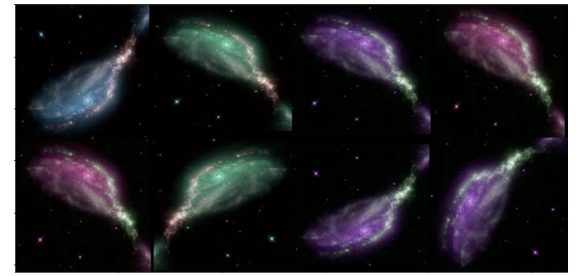
\includegraphics[width=0.5\textwidth]{Images/augmented-sample.png}
    \caption{Data-augmentation (Eight images out of one!)}
    \label{fig:enter-label}
\end{figure}

We resized all images to \(128 \times 128\) pixels and combined them into our final dataset, which includes:

\begin{itemize}
    \item 1001 Spiral images
    \item 991 Irregular images
    \item 828 Elliptical images
    \item 800 Invalid images
\end{itemize}

We applied PCA to the images for dimensionality reduction. Image preprocessing involved flattening images and Z-score normalization. Each image was represented as a vector of size \(128 \times 128 \times 3 = 49152\). The observed total variance after normalization was slightly less than the theoretical expectation (49116), confirming Hypothesis 0.1.

To preserve approximately 95\% of the variance, we determined that using 256 Principal Components (PCs) was sufficient based on the explained variance plot (Figure 1.2).

After PCA, we split the data into 70\% training and 30\% validation sets. Figures 1.3 and 1.4 illustrate sample images before and after PCA, respectively.

\begin{figure}[H]
    \centering
    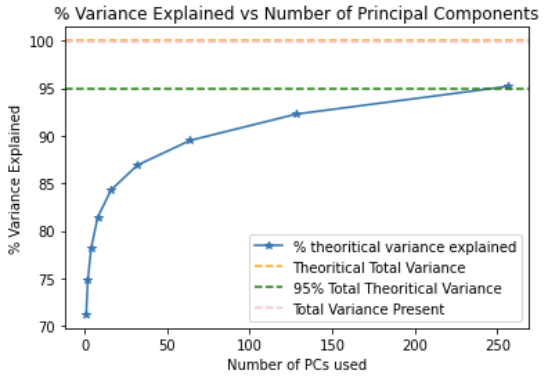
\includegraphics[width=0.5\textwidth]{Images/percent-variance.png}
    \caption{Percent of variances explained by number of Principal Components}
\end{figure}

\begin{figure}[H]
    \centering
    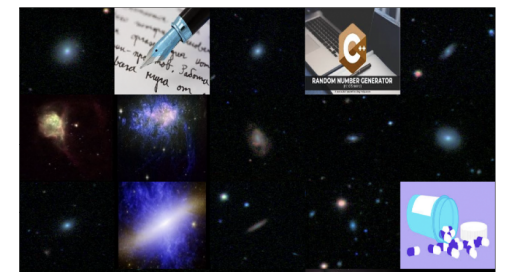
\includegraphics[width=0.5\textwidth]{Images/before-pca.png}
    \caption{Sample images before applying PCA (high dimension)}
\end{figure}

\begin{figure}[H]
    \centering
    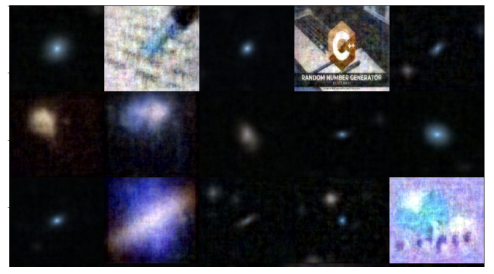
\includegraphics[width=0.5\textwidth]{Images/after-pca.png}
    \caption{Same images after applying PCA (reduced dimension)}
\end{figure}

We trained Support Vector Machine (SVM) and Random Forest classifiers on the dataset. For SVM, a linear kernel provided the highest accuracy. The Random Forest classifier used the Gini index as the split criterion with 100 trees.

We also trained a Multi-Layer Perceptron (MLP) using Keras with TensorFlow backend. Hyperparameter tuning involved selecting an adaptive momentum optimizer, dropout rate, and layer configuration. Training and validation learning curves for the MLP are shown in Figure 1.5.

\begin{figure}[H]
    \centering
    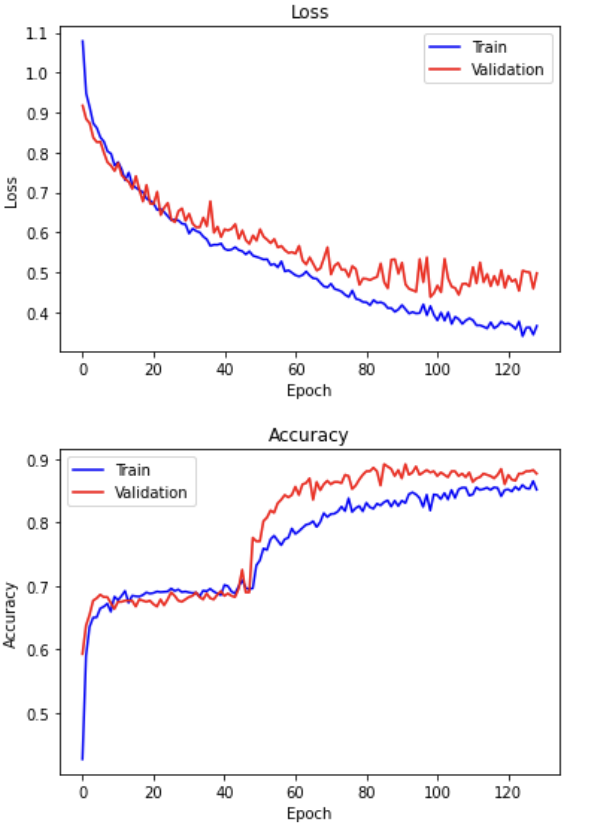
\includegraphics[width=0.5\textwidth]{Images/loss-accuracy-mlp.png}
    \caption{Loss and Accuracy plots generated for training and validation in MLP}
\end{figure}

Similarly, we trained a Convolutional Neural Network (CNN) with optimized hyperparameters. The best-performing CNN model had 4 layers with rectified linear activation and achieved training and validation accuracy depicted in Figure 1.6.

\section{Results}

For our experimental run with a linear SVM, we achieved $86.13 \%$ accuracy, with the precision, recall, and F1-scores for this model displayed in Table 1.1. Moreover, using the random forest method, we achieved $92.06 \%$ accuracy with the aforementioned metrics for it displayed in Table 1.1 as well. We compare this to the result found in the experiment done by Calleja and Fuentes who also performed PCA and then random forest, which received an accuracy of $91.64 \%$. The difference between our experiment and the experiment done by Calleja and Fuentes is that we include a fourth class of classification, the invalid category. Calleja and Fuentes use only three classes: elliptical, spiral, and irregular. Regardless of this difference, we found that our random forest classifier was able to distinguish invalid images as well while achieving a slightly higher accuracy. We found that the accuracy of our random forest run was higher than that of our linear SVM, thus corroborating our Hypothesis 2.

\begin{figure}[H]
    \centering
    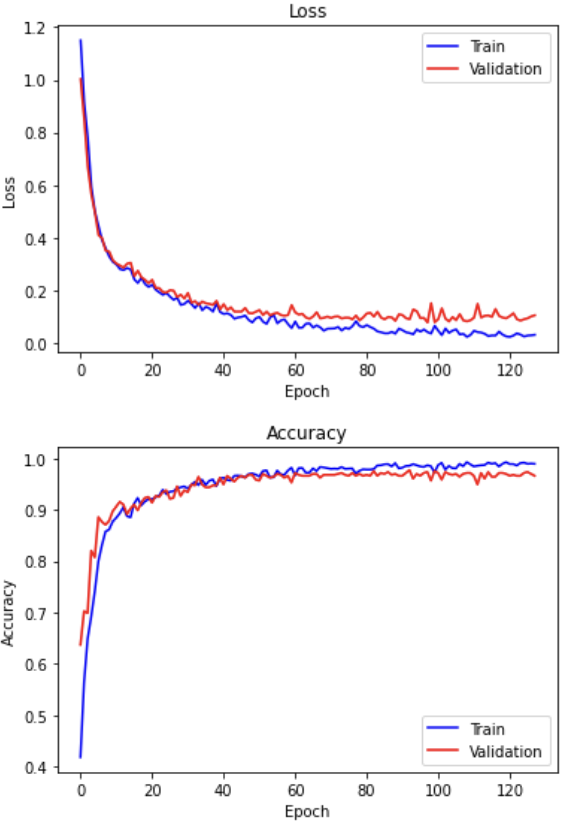
\includegraphics[width=0.5\textwidth]{Images/loss-accuracy-cnn.png}
    \caption{Loss and Accuracy plots generated for training and validation in Convolutional Neural Nets}
\end{figure}

The below Figure 1.9 shows the predictions of each image along with the actual class label. Table 1.1 displays the classification reports with precision, recall and F1-score for SVM classifier and Random Forest Classifier.

In Figure 1.7 and Figure 1.8, we see the ROC curve for the linear SVM and random forest classifiers, respectively. The ROC curves further evince that the random forest classifier achieves better performance than the linear SVM. We can see that in Figure 1.8, the true positive rate is very close to 1.0 while the false positive rate is very close to 0.0 for classes 2 and 3 compared to the curves in Figure 1.7 for classes 2 and 3 . We can also see that the curves for classes 0 and 1 are closer to the $(0,1)$ point of the curve in Figure 1.8 than in Figure 1.7.

\begin{table}
    \centering
    \caption{Classification Report of Linear SVM and Random Forest $P$-Precision, $R$ - Recall, F1 - F1 Score, WA - Weighted Average}
    
    \begin{tabular}{|c|c|c|c|c|c|c|}
    \hline
     & \multicolumn{3}{|c|}{Linear SVM} & \multicolumn{3}{|c|}{Random Forest} \\
    \hline
    Class & $\mathrm{P}$ & $\mathrm{R}$ & $\mathrm{F} 1$ & $\mathrm{P}$ & $\mathrm{R}$ & $\mathrm{F} 1$ \\
    \hline
    0 & 0.79 & 0.88 & 0.83 & 0.89 & 0.90 & 0.90 \\
    \hline
    1 & 0.86 & 0.81 & 0.84 & 0.92 & 0.85 & 0.89 \\
    \hline
    2 & 0.86 & 0.94 & 0.90 & 0.91 & 0.97 & 0.94 \\
    \hline
    3 & 0.97 & 0.80 & 0.88 & 0.96 & 0.97 & 0.96 \\
    \hline
    WA & 0.85 & 0.85 & $\mathbf{0 . 8 6}$ & 0.92 & 0.92 & $\mathbf{0 . 9 2}$ \\
    \hline
    \end{tabular}
    
\end{table}

\begin{figure}[H]
    \centering
    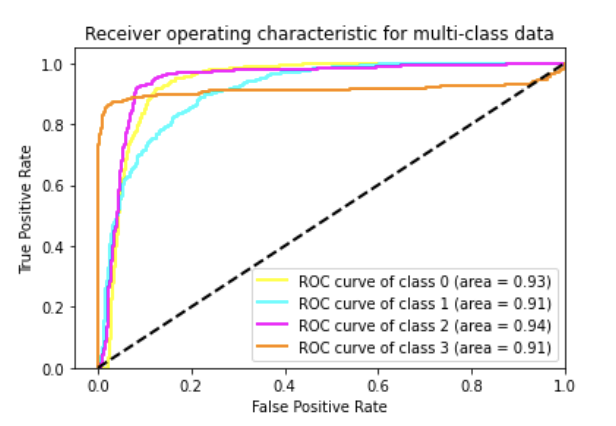
\includegraphics[width=0.5\textwidth]{Images/ROC-curve-SVM.png}
    \caption{ROC curve for the linear SVM}
\end{figure}

\begin{figure}[H]
    \centering
    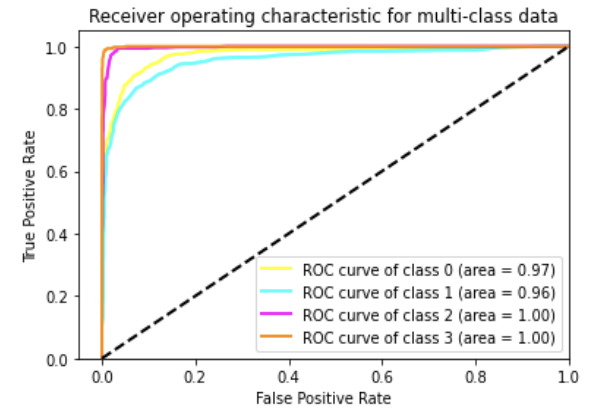
\includegraphics[width=0.5\textwidth]{Images/ROC-curve-rfc.png}
    \caption{ROC curve for the Random Forest Classifier}
\end{figure}

Our MLP model achieved classification accuracy of about $\mathbf{8 7 \%}$. We have shown the loss and accuracy plots for MLP in Figure 1.5. We also provide the classification report for our MLP model in Table 1.2. An interesting feature of our accuracy plot in Figure 1.5 is that the validation accuracy ends up being greater than the training accuracy as model training continues. However, it is still within the margin of error and is a weak indication of generalizable performance. In Figure 1.9, we show a sample of images with their actual and predicted class that resulted from the MLP model.

% Table 1.2: Classification Report of MLP and CNN

\begin{center}[H]
$\begin{array}{|c|c|c|c|c|c|c|}\hline&&\mathbf{MLP}&&&\mathbf{CNN}&\\\hline\text{Class}&\text{P}&\text{R}&\text{F1}&\text{P}&\text{R}&\text{F1}\\\hline0&0.80&0.85&0.82&0.95&0.98&0.96\\\hline1&0.86&0.88&0.82&0.97&0.93&0.95\\\hline2&0.93&0.89&0.91&0.98&0.97&0.97\\\hline3&0.88&0.96&0.92&0.97&0.98&0.98\\\hline\text{WA}&0.87&0.90&\textbf{0.87}&0.97&0.97&\textbf{0.97}\\\hline\end{array}$
\end{center} 

\begin{figure}[H]
    \centering
    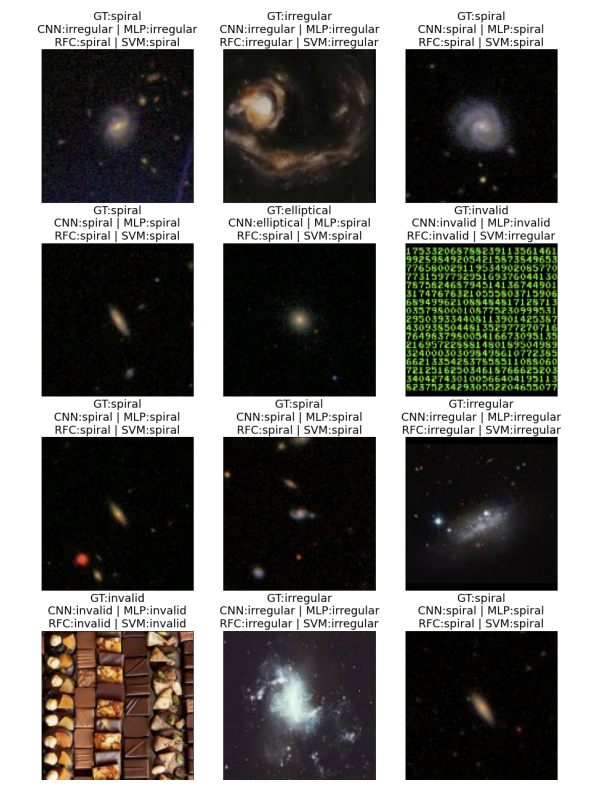
\includegraphics[width=0.5\textwidth]{Images/sample-images.png}
    \caption{Sample images with their actual and predicted class for RFC, SVM,MLP and CNN model}
\end{figure}

% GT:spiral\\
% CNN:irregular | MLP:irregu\\
% RFC:spiral | SVM:spiral

% GT:spiral\\
% CNN:spiral | MLP:spiral\\
% RFC:spiral | SVM:spiral

% GNN:ellipticlical | MLP:spiral

% \begin{center}
% \includegraphics[max width=\textwidth]{2024_05_01_50074901ee5ad42c853eg-6(1)}
% \end{center}

% CNN:invalid | MLP:invalic

% \begin{center}
% \includegraphics[max width=\textwidth]{2024_05_01_50074901ee5ad42c853eg-6}
% \end{center}

% GTi:rregular\\
% NN:\\
% Cirregular I MLP:irregula\\
% a RFC:irregular $\mid$ SVM:irregular

% CNN:spiral | MLP:spir

% RFC:spiral | SVM:spiral

% Figure 1.9 Sample images with their actual and predicted class for $R F C, S V M, M L P$ and CNN model

Our CNN model performed at an accuracy of $97 \%$. We have shown the loss and accuracy plots above in Figure 1.6. We also provide the classification report for our CNN model in Table 1.2. It is observed that as the hidden layers in the model are increased, the accuracy of the model increases. In Figure 1.9, we show a sample of images with their actual and predicted class that resulted from the CNN model.
\section{Conclusions}

Through our experiments, we have explored various machine learning and deep learning models for automating the identification of galaxies based on image data. Our findings demonstrate that the CNN model achieved the highest performance on our dataset consisting of elliptical, spiral, irregular, and invalid images, achieving a classification accuracy of \(97\%\). While the CNN model showed superior performance, there is potential to further enhance accuracy by leveraging ensemble methods from traditional machine learning classifiers.

We believe that the techniques developed for galaxy image classification can be extended to other astronomical data types, such as nebulae, star clusters, or images containing multiple astronomical objects. The models we have created hold practical value for various algorithms in astronomy.

In conclusion, we introduce a new benchmark for galaxy image classification and highlight our best-performing model, the CNN, achieving a remarkable \(97\%\) classification accuracy, surpassing previous attempts by at least \(5\%\).

During this project, we gained valuable experience in various machine learning tasks, including:

\begin{itemize}
    \item Web-scraping images using SDSS APIs and astropy
    \item Image data augmentation with imgaug
    \item Applying PCA on images using scikit-learn
    \item Implementing Random Forests and SVMs using scikit-learn
    \item Building MLP and CNN models using Keras
    \item Generating classification reports and ROC curves using matplotlib and scikit-learn
    \item Visualizing results with matplotlib
\end{itemize}
\section*{References}
\label{sec:References}

[1] Pedregosa, F., Varoquaux, Gael, Gramfort, A., Michel, V., Thirion, B., Grisel, O., ... others. (2011). Scikit-learn: Machine learning in Python. Journal of Machine Learning Research, 12(Oct), 2825-2830.

[2] Chollet, F., \& others. (2015). Keras. GitHub. Retrieved from \href{https://github.com/fchollet/keras}{\textcolor{blue}{https://github.com/fchollet/keras}}

[3] Hunter, J. D. (2007). Matplotlib: A 2D graphics environment. Computing in Science \&amp; Engineering, 9(3), 90-95.

[4] Alexander B. Jung. (2018). imgaug. \href{https://github.com/aleju/imgaug}{\textcolor{blue}{https://github.com/aleju/imgaug}}.

[5] Hector Robles, Hugo Soto. (2019). Identifying Galaxies Using the Deep Learning Reference Stack. \href{https://01.org/blogs/2019/identify-galaxies-using-deep}{\textcolor{blue}{https://01.org/blogs/2019/identify-galaxies-using-deep}} -learning-reference-stack

[6] Price-Whelan A., et al. The Astropy Project: Building an open-science project and status of the v2. 0 core package. The Astronomical Journal. 2018;156(3):123.
{
    \small
    \nocite{*}
    \bibliographystyle{ieeenat_fullname}
    % \bibliography{main}
}

% WARNING: do not forget to delete the supplementary pages from your submission 
% \input{sec/X_suppl}

\end{document}
